% Blabla Matériel et Méthodes

In this part, will be detailed all the hardware, software and methods used to carry out simulations. 

\section{Hardware and Software}

    As this internship is 100\% digital, a good comuter is required. A personal computer (MacBook Air M1) as well as a computer provided by the laboratory (under Ubuntu) will be the main equipment for this internship. \medskip

    The main softwares are the following ones:

    \begin{enumerate}[\hspace{3em}$\bullet$]
        \item \textbf{Visual Studio Code (VS Code)}: a source-code editor developed by Microsoft.
        \item \textbf{Large-scale Atomic/Molecular Massively Parallel Simulator (LAMMPS)}: a molecular dynamics programm (coded in \verb|C++|) from \href{http://www.sandia.gov}{Sandia National Laboratories}.
        \item \textbf{Ovito}: a visualization and analysis software for output data generated in molecular dynamics. 
        \item \textbf{Perseus GRICAD}: high performance computing and storage platforms.  
    \end{enumerate}

    \subsection{LAMMPS}

        LAMMPS is an open-source molecular dynamic code with a focus on materials modeling. It provides potentials for solid-state materials (metals and semiconductors). It can be used to model atoms or, more generically, as a parallel particle simulator at the atomic, meso, or continuum scale. \medskip

        LAMMPS does not have any graphic interface which makes the handholding not that easy. The input code is written is \verb|.txt| files thats are compilled through a \verb|Makefile| called with a \verb|bash| command : \verb|lmp_serial -in input.file.txt|.
        
        LAMMPS provides a \verb|log.lammps| file as output. All the behaviour of the script (output values, warnings, errors \dots) is written in this file. However, with specific commands, this software can provide other outfile such as a \verb|dump.test| file, which will be useful to have a visualization of the material behaviour. \medskip

        Here is a quick recap : 

        \begin{center}
            \captionsetup{type=figure}
            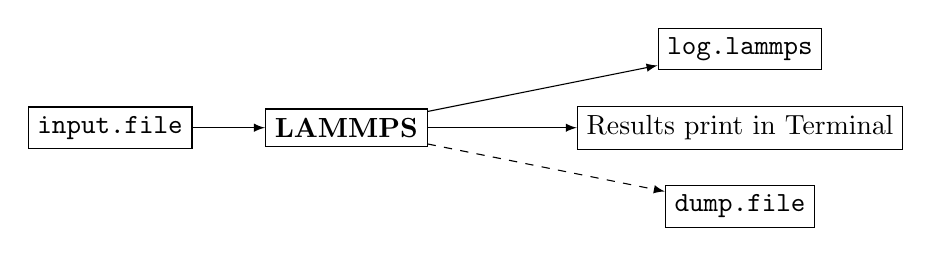
\begin{tikzpicture}
                \node[draw](I) at (0,0) {\verb|input.file|};
                \node[draw](L) at (3,0) {\textbf{LAMMPS}};
                \node[draw](LOG) at (8,1) {\verb|log.lammps|};
                \node[draw](RES) at (8,0) {Results print in Terminal};
                \node[draw](D) at (8,-1) {\verb|dump.file|};
                \draw[->,>=latex] (I) -- (L);
                \draw[->,>=latex] (L) -- (LOG);
                \draw[->,>=latex] (L) -- (RES);
                \draw[->,>=latex,dashed] (L) -- (D);
            \end{tikzpicture}
            \captionof{figure}{LAMMPS operation}
        \end{center}

    \subsection{Ovito}
        
        Ovito is a scientific visualization and data analysis tool for atomistic and other particle-based models. The community edition is free of charge under an open source license. Ovito has a Pro version which is a powerful extension with extended analysis toolset, visualization capabilities and automation with the \verb|Python| integration. For this intership, the community edition is used. \medskip

        Ovito will be used to visualize the behaviour of the atoms (mainly their position and velocity along the x,y and z axes). It will help to have a first sight of the simulation to see if there is no inconsitent behaviours before going deeper in the process.

        The visualization is based on the \verb|dump.file| that LAMMPS is producing. So here is the final scheme : 

        \begin{center}
            \captionsetup{type=figure}
            \begin{tikzpicture}
                \node[draw](I) at (0,0) {\verb|input.file|};
                \node[draw](L) at (3,0) {\textbf{LAMMPS}};
                \node[draw](LOG) at (8,1) {\verb|log.lammps|};
                \node[draw](RES) at (8,0) {Results print in Terminal};
                \node[draw](D) at (8,-1) {\verb|dump.file|};
                \node[draw](O) at (8,-2) {\textbf{Ovito}};
                \node[draw](OEX) at (5,-4) {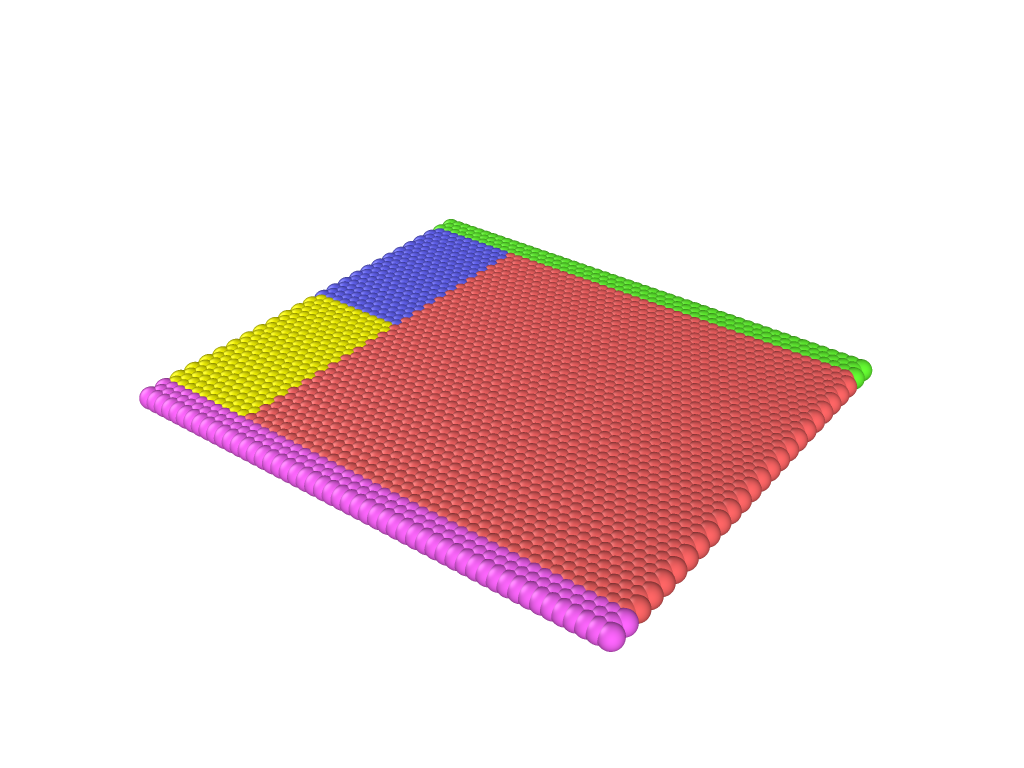
\includegraphics[scale = 0.1]{ovito_ex.png}};
                \draw[->,>=latex] (I) -- (L);
                \draw[->,>=latex] (L) -- (LOG);
                \draw[->,>=latex] (L) -- (RES);
                \draw[->,>=latex,dashed] (L) -- (D);
                \draw[->,>=latex] (D) -- (O);
                \draw[->,>=latex] (O) -| (OEX);
            \end{tikzpicture}
            \captionof{figure}{Final Operation Scheme}
        \end{center}
    
    \subsection{Perseus GRICAD}

        GRICAD offers intensive computing and data processing infrstructures to answer the needs of scientists. This tool provides an access to computing, grid, cloud, notebook and associated storage platforms. Moreover, an user support with assitance is opened. These infrastructures are open to all members of the scientific communities of the Grenoble site, as well as to their external collaborators. To have an access to this computing tool, a Perseus account is required. Once the Perseus account is created, you need to be member of the project to run your scripts. For this internship, the project is \verb|pr-atosimul|. \medskip

        GRICAD provides four computing culsters that are different (each cluster have their own hardware and configuration). Cluster access is normally done using a \verb|SSH Client| (Secure Shell Protocol) \cite{1}. However, \gls{SSH} servers are vulnerable to scans and attacks so, for security reasons, it is not possible to let the clusters be directly accessed from the internet. GRICAD provides two \gls{SSH} gateways that are more secure than the clusters. So the login method is to first, login to an \gls{SSH} gateway and the login to the targeted cluster : 

        \begin{center}
            \captionsetup{type=figure}
            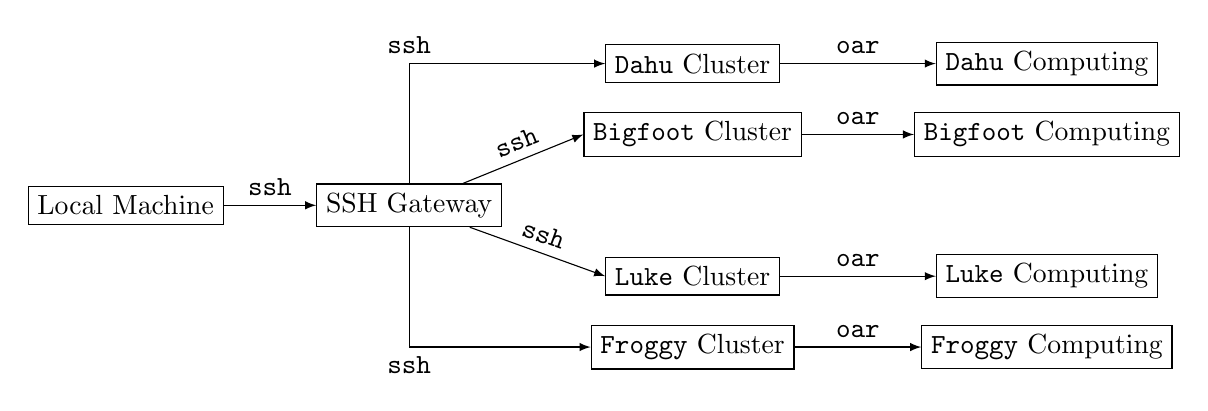
\begin{tikzpicture}[scale = 0.9]
                \node[draw](LOC) at (0,0) {Local Machine};
                \node[draw](SSH) at (4,0) {SSH Gateway};
                \node[draw](DAHU) at (8,2) {\verb|Dahu| Cluster};
                \node[draw](BIGF) at (8,1) {\verb|Bigfoot| Cluster};
                \node[draw](LUKE) at (8,-1) {\verb|Luke| Cluster};
                \node[draw](FROG) at (8,-2) {\verb|Froggy| Cluster};
                \node[draw](DAHUC) at (13,2) {\verb|Dahu| Computing};
                \node[draw](BIGFC) at (13,1) {\verb|Bigfoot| Computing};
                \node[draw](LUKEC) at (13,-1) {\verb|Luke| Computing};
                \node[draw](FROGC) at (13,-2) {\verb|Froggy| Computing};
                \draw[->,>=latex] (LOC) -- (SSH) node[midway,above]{\verb|ssh|};
                \draw[->,>=latex] (SSH) |- (DAHU) node[midway,above,sloped]{\verb|ssh|};
                \draw[->,>=latex] (SSH) -- (BIGF.west) node[midway,above,sloped]{\verb|ssh|};
                \draw[->,>=latex] (SSH) -- (LUKE.west) node[midway,above,sloped]{\verb|ssh|};
                \draw[->,>=latex] (SSH) |- (FROG) node[midway,below,sloped]{\verb|ssh|};
                \draw[->,>=latex] (DAHU) -- (DAHUC) node[midway,above]{\verb|oar|};
                \draw[->,>=latex] (BIGF) -- (BIGFC) node[midway,above]{\verb|oar|};
                \draw[->,>=latex] (LUKE) -- (LUKEC) node[midway,above]{\verb|oar|};
                \draw[->,>=latex] (FROG) -- (FROGC) node[midway,above]{\verb|oar|};
            \end{tikzpicture}
            \captionof{figure}{SSH cluster access schema}
        \end{center}
        
        Those two \gls{SSH} gateways (called \verb|Rotule| and \verb|Trinity|) are grouped under a single DNS : \verb|access-gricad.univ-grenoble-alpes.fr|. This allows for load balancing on these two machines. Moreover, if one server came to fail, the other one is still available for computing. 
        
        The submission work for computing is made through a \verb|run.oar| file. It is a \verb|bash| script that provides the number of nodes and cores of the processor wanted by the user, the walltime (max time of computing), the name of some output files and then commands to run external scripts. A script is given in the \ref{section:run_oar} appendix.

        Then, all the output files are stored on the cluster. To visualize them through Ovito for instance, a File Transfer Protocol Secure (FTPS) is used. 


\section{Methods}

    The aim is to make predictions about the behavior of cracks using a Machine Learning program. The algorithm will have to learn from the numerous simulations. It is therefore crucial that these input data are correct in order to limit the error on the predictions at the output of the program. So the first part of this internship is to work on the limit and initial conditions in order to have correct simulations.

    \subsection{The Theory}

        As mentionned before, this internship is a multiscale analysis. So, it focuses on Molecular Dynamic for the small scale and Fracture Mechanic for the large scale. \medskip

        \subsubsection{Fracture Mechanics}
            Here is a simplified scheme of a fracture : 
                \begin{center}
                    \captionsetup{type=figure}
                    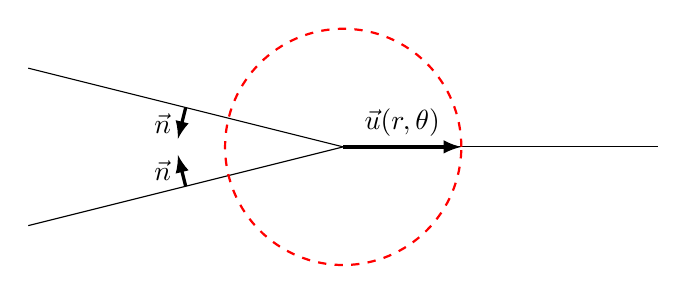
\begin{tikzpicture}
                        \draw (0,1) -- (4,0) -- (0,-1);
                        \draw (4,0) -- (8,0);
                        \draw[->,>=latex,very thick] (2,0.5) -- (1.9,0.1) node[midway,below,left]{$\vec{n}$};
                        \draw[->,>=latex,very thick] (2,-0.5) -- (1.9,-0.1) node[midway,below,left]{$\vec{n}$};
                        \draw[red, thick, dashed] (4,0) circle (1.5);
                        \draw[->,>=latex,very thick] (4,0) -- (5.5,0) node[midway,above]{$\vec{u}(r,\theta)$};
                    \end{tikzpicture}
                    \captionof{figure}{Simplified fracture scheme}
                \end{center}
            
            A crack is defined by a discontinuity in the potential $\vec{u}$ and that there is no stress on the free surfaces $(\vec{T} = \vec{0})$. According to Fracture Mechanic, the dashed red circle corresponds to the \gls{cohesive zone} model. Outside this area, the surfaces are free of effort: $\vec{T} = \underline{\underline{\sigma}}\cdot\vec{n} = \vec{0}$. This is not the case in the \gls{cohesive zone} where we have an interatomic potential $\vec{u}$ defined as $\vec{u}(r,\theta) = f(r)\times g(\theta)\cdot\vec{u_r}$. \medskip
            
            According to T.L. Anderson \cite{2}, locally (so when $r\rightarrow 0$), we have :
            $$
            \vec{u} = \frac{K_1}{2\mu}\sqrt{r}f_{XY}(\theta) \quad\text{where}\quad K_1 = \text{a loading parameter}
            $$
            $K_1$ depends mainly on the type of crack (on the side, central, in tension, in traction...) and $f_{XY}$ is a function that depends on $X$ and $Y$ which are the plan coordinates.\medskip

            The interatomic potential induces an interatomic force $\vec{F} = \nabla \vec{u}$ which (\textit{on the figure below, $T$ is the stress vector defined as $\vec{T} = \frac{\sum\vec{f}_i}{S}$ where $S$ corresponds to the surface}). 

            \begin{center}
                \captionsetup{type=figure}
                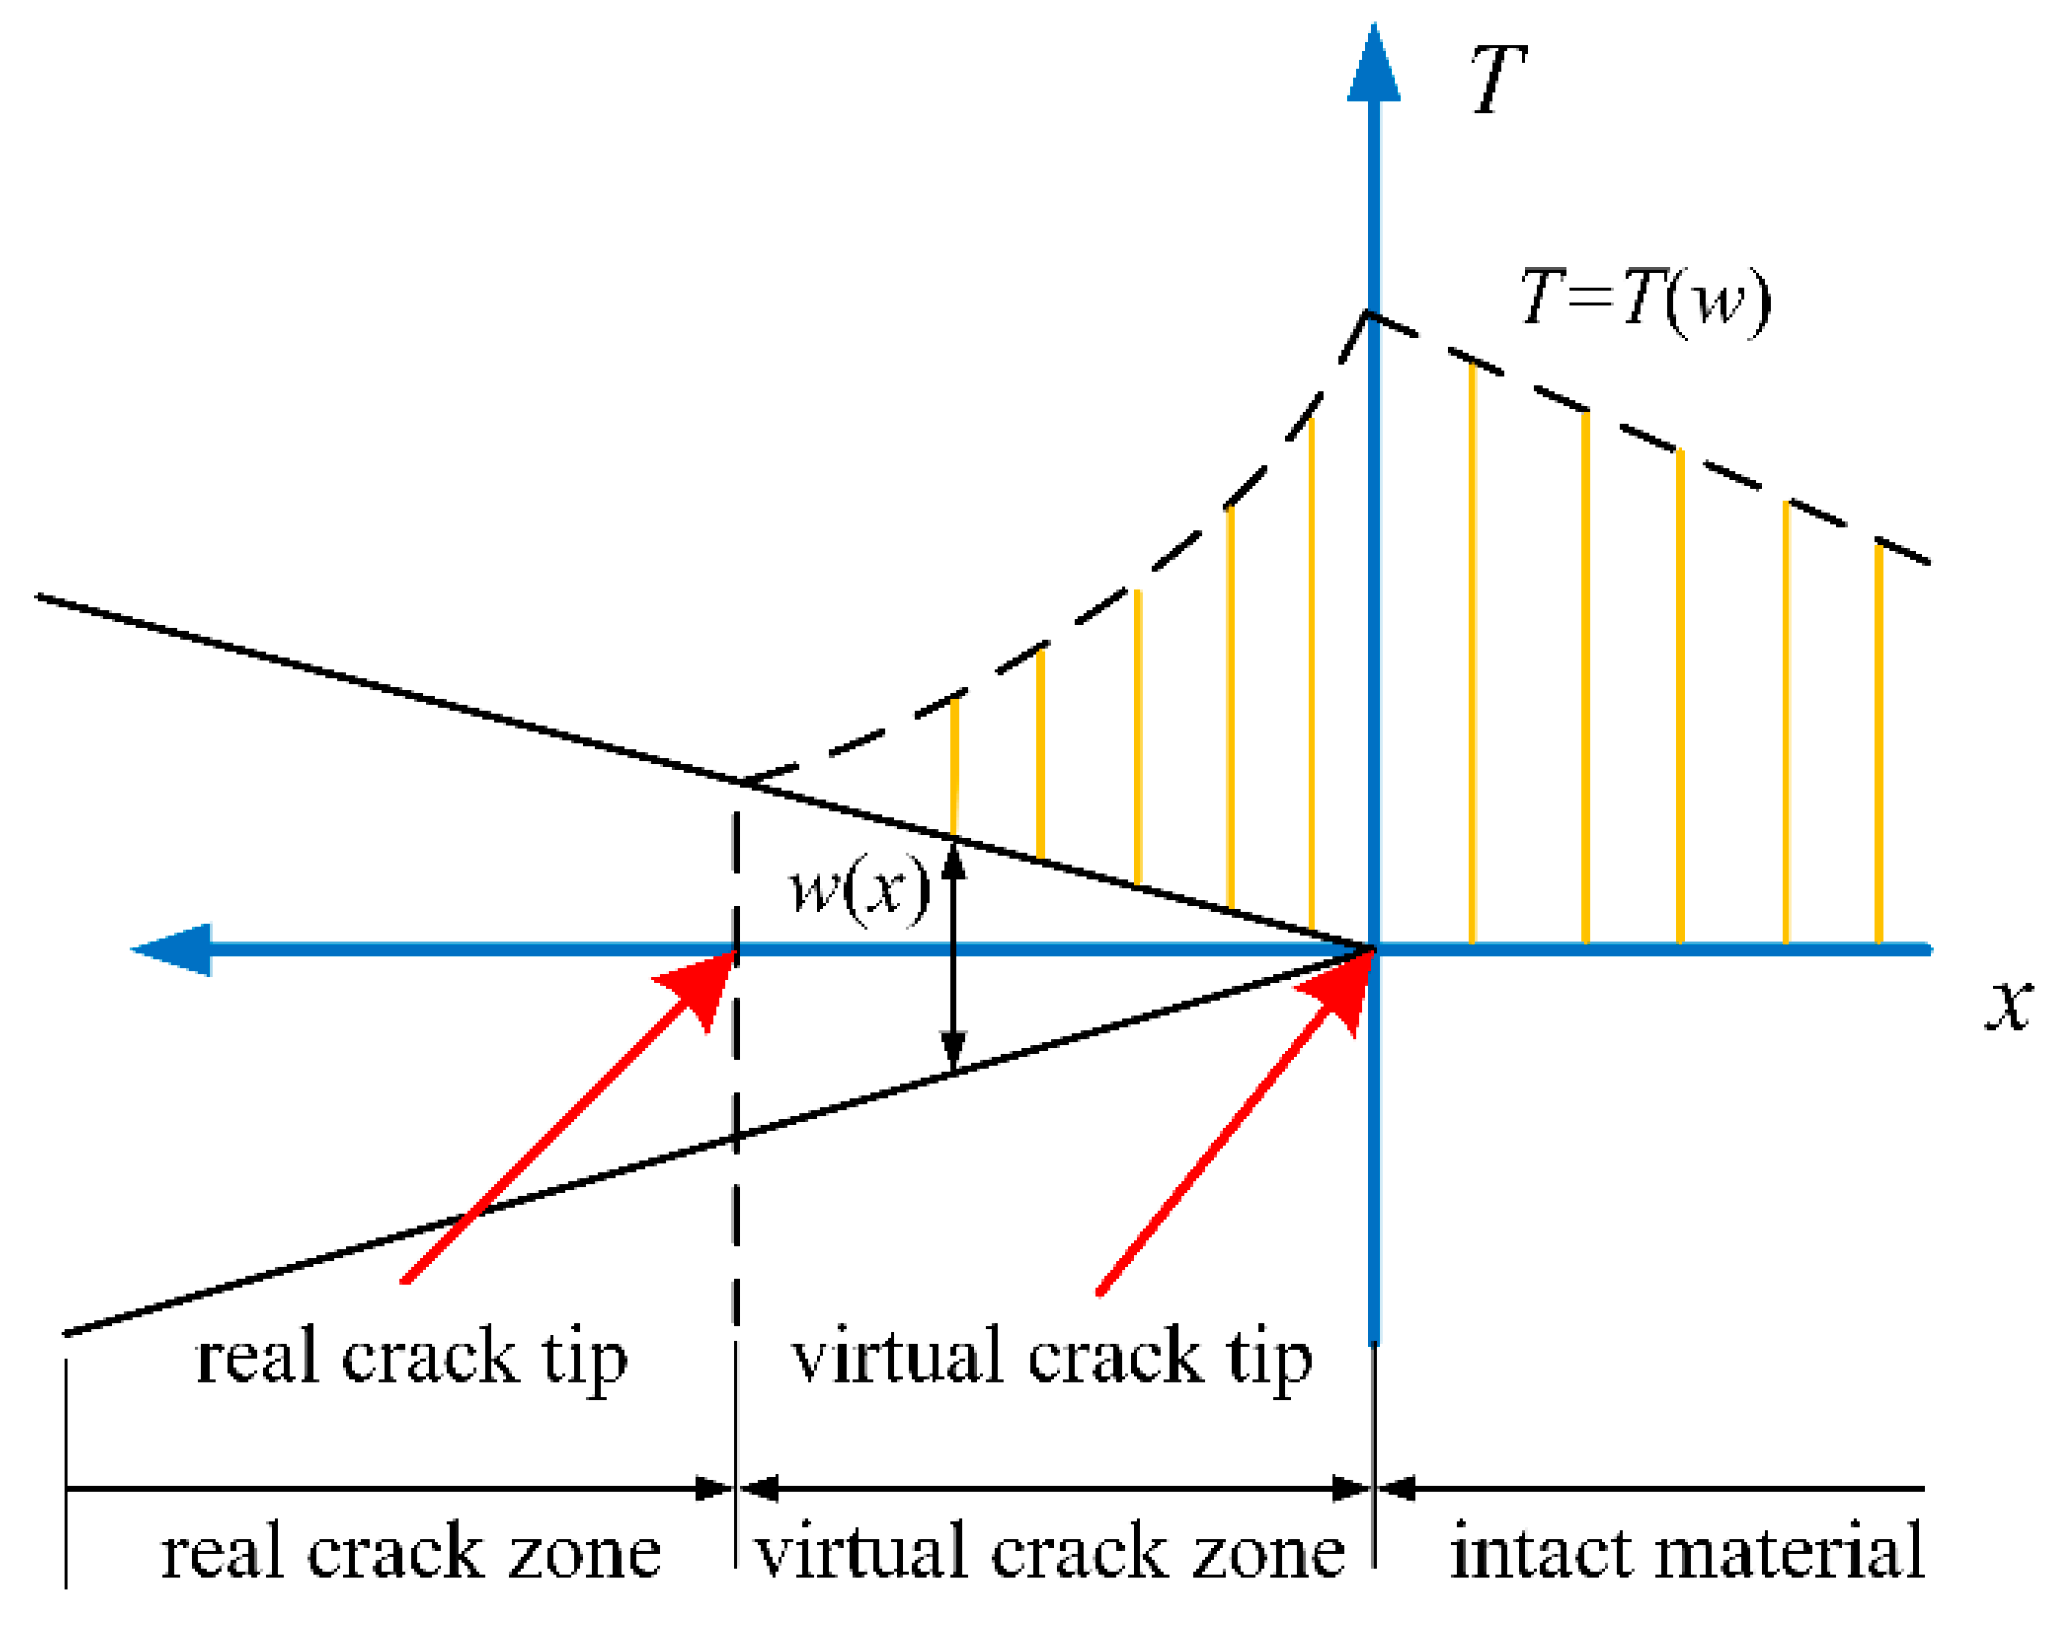
\includegraphics[scale = 0.1]{inter_force.png}
                \captionof{figure}{Interatomic force $\vec{F}$ \cite{3}}
            \end{center}
            
            We can define $a_0$ which is the distance from the virtual crack tip where the interatomic force is zero : $\Delta = r - a_0$. 
            
            So, we have the following criteria : 

            $$
            \left\lbrace\begin{array}{l}
                \Delta < 0 \implies f < 0 \implies \text{atoms repulsion}\\
                \Delta > 0 \implies f > 0 \implies \text{atoms attraction}
            \end{array}\right.
            $$
            \medskip

            This \gls{cohesive zone} implies a difficult problem to resolve during a tensile test. The solution is to split the problem into two independent and simpler to solve problems. The first problem is a tensile test with a crack on the side without taking into account the \gls{cohesive zone} model. The second problem is to take the \gls{cohesive zone} model but without traction. To make the tests independent, there are two different loading parameters $K_1$. In the case of the first test, it is a crack opening parameter $K_{1_{opening}}$. In the case of the second test, it is a crack closing parameter $K_{1_{closing}}$.

            \begin{center}
                \captionsetup{type=figure}
                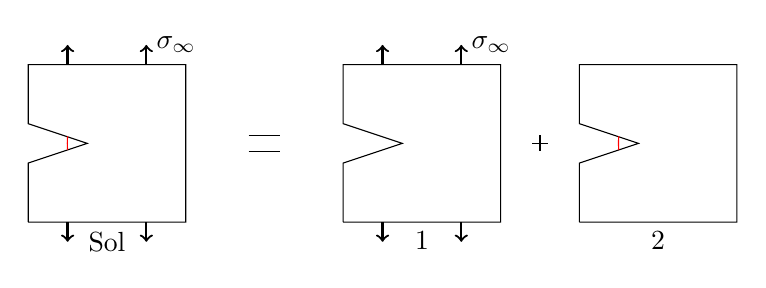
\begin{tikzpicture}
                    % Première figure 
                    \draw (0,0) -- (0,0.75) -- (0.75,1) -- (0,1.25) -- (0,2) -- (2,2) -- (2,0) -- (0,0) node[midway, below]{Sol};
                    \draw[thick,->] (0.5,2) -- (0.5,2.25);
                    \draw[thick,->] (1.5,2) -- (1.5,2.25) node[right]{$\sigma_{\infty}$};
                    \draw[thick,->] (0.5,0) -- (0.5,-0.25);
                    \draw[thick,->] (1.5,0) -- (1.5,-0.25);
                    \draw[red] (0.5,1.09) arc (175:185:1cm);
        
                    % égal
                    \draw (2.8,1.1) -- (3.2,1.1);
                    \draw (2.8,0.9) -- (3.2,0.9);
        
                    % Deuxième figure 
                    \draw (4,0) -- (4,0.75) -- (4.75,1) -- (4,1.25) -- (4,2) -- (6,2) -- (6,0) -- (4,0) node[midway, below]{1};
                    \draw[thick,->] (4.5,2) -- (4.5,2.25);
                    \draw[thick,->] (5.5,2) -- (5.5,2.25) node[right]{$\sigma_{\infty}$};
                    \draw[thick,->] (4.5,0) -- (4.5,-0.25);
                    \draw[thick,->] (5.5,0) -- (5.5,-0.25);
        
                    % +
                    \draw (6.5,1.1) -- (6.5,0.9);
                    \draw (6.4,1) -- (6.6,1);
        
                    % Deuxième figure 
                    \draw (7,0) -- (7,0.75) -- (7.75,1) -- (7,1.25) -- (7,2) -- (9,2) -- (9,0) -- (7,0) node[midway, below]{2};
                    \draw[red] (7.5,1.09) arc (175:185:1cm);
                \end{tikzpicture}
                \captionof{figure}{Problem splitting}
            \end{center}
        
            Then, in order to calculate the crack propagation using fracture mechanics, a propagation criteria has been demonstrated by Alan Arnold Griffith \cite{4} in his paper. He demonstrated for a tensile test charged with $\sigma_{\infty}$, with $G$ the energy per unit of free area, $A$ the free surface, $W$ the crack work and $a$ the crack lenght, that:

            $$
            \frac{\partial W}{\partial A} = \frac{W\left[(2(a + da))\right] - W\left[(2a)\right]}{dA} = 2\gamma
            $$

            Moreover, $\frac{\partial W}{\partial A}$ corresponds to the consumed energy to create an additional free surface. So, as long as $G < \frac{\partial W}{\partial A}$, there is no crack propagation. However, when $G = 2\gamma$, there is propagation iniation.\medskip

            That is how we calculate fracture propagation in materials according to fracture mechanics. But, we cannot really go deeper in the virtual crack zone and understand all the atomic interactions in the \gls{cohesive zone}. To have a better understanding of potentials and crack propgation, we need to look closer and use \gls{molecular dynamic}.
        
        \subsubsection{Molecular Dynamics}
            
            \Glspl{molecular dynamic} is a numerical method that resolver Newton's equation of motion $\vec{F} = \frac{d}{dt}(m\vec{v})$ for system of interacting. As the atoms are allowed to interact thanks to interatomic potentials for a fixed period of time, it gives the dynamic evolution of the system. \medskip

            Here is a simplified schema of a \gls{molecular dynamic} progam (such as LAMMPS) : 

            \begin{center}
                \captionsetup{type=figure}
                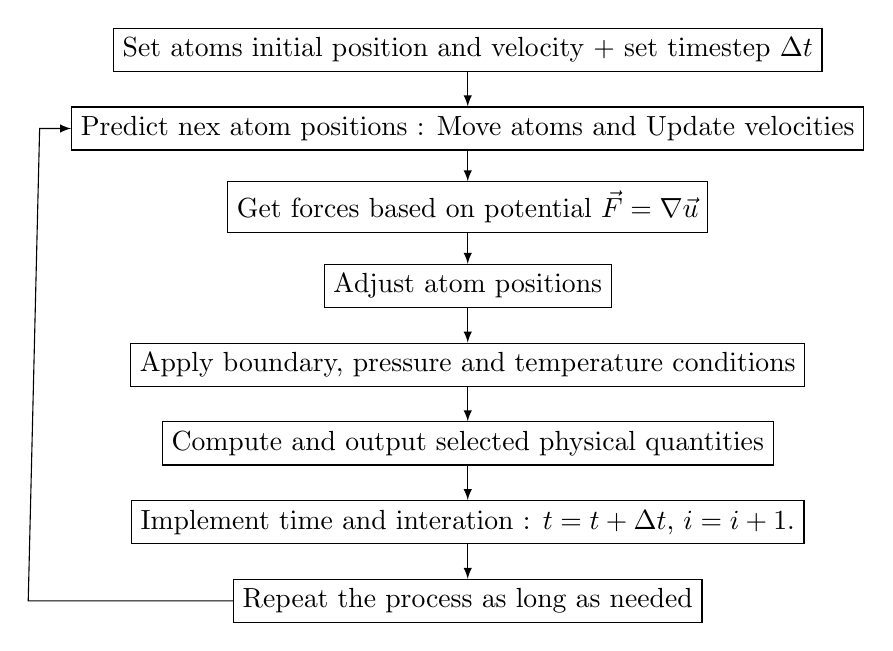
\begin{tikzpicture}
                    \node[draw](A) at (0,0) {Set atoms initial position and velocity + set timestep $\Delta t$};
                    \node[draw](B) at (0,-1) {Predict nex atom positions : Move atoms and Update velocities};
                    \node[draw](C) at (0,-2) {Get forces based on potential $\vec{F} = \nabla\vec{u}$};
                    \node[draw](D) at (0,-3) {Adjust atom positions};
                    \node[draw](E) at (0,-4) {Apply boundary, pressure and temperature conditions};
                    \node[draw](F) at (0,-5) {Compute and output selected physical quantities};
                    \node[draw](G) at (0,-6) {Implement time and interation : $t = t + \Delta t$, $i = i + 1$.};
                    \node[draw](H) at (0,-7) {Repeat the process as long as needed};
                    \coordinate[shift={(-2.6cm,0)}] (n) at (H.west);
                    \coordinate[shift={(-4mm,0)}] (m) at (B.west);
                    \draw[->,>=latex] (A) -- (B);
                    \draw[->,>=latex] (B) -- (C);
                    \draw[->,>=latex] (C) -- (D);
                    \draw[->,>=latex] (D) -- (E);
                    \draw[->,>=latex] (E) -- (F);
                    \draw[->,>=latex] (F) -- (G);
                    \draw[->,>=latex] (G) -- (H);
                    \draw[->,>=latex] (H) -- (n) -- (m) -- (B);
                \end{tikzpicture}
                \captionof{figure}{Simplified schema of a molecular dynamic program}
            \end{center}

            The engineering of a \gls{molecular dynamic} algorithm should account for the available computational power of the machine. That is why parameters such as timestep, simulation box size, number of atoms, potential\dots are wisely choose to have a correct computational time. Thoose simualtions requires sometimes high computational power to output some results. That is why a calculating computer is used during this internship. The type of system is also an important parameter to take into consideration. Only microcanonical (\gls{NVE}), canonical (\gls{NVT}) and isothermal-isobaric (\gls{NPT}) ensembles are used for simulations. 

            In the microcanonical ensemble, the system is totally isolated from changes in moles (N), volumes (V) and energy (E). It is linked with an \gls{adiabatic} process without heat exchange. 

            In the canonical ensemble, the amount of atoms (N), volume (V) and temperature (T) are conserved. In a \gls{NVT} system, the energy is exchanged with a thermostat. There are several thermostat algorithm and methods. 

            In the isothermal-isobaric ensemble, the amount of atoms (N), pressure (P) and temperature (T) are conserved. Compared to the \gls{NVT} ensemble, a barostat is needed in addition to a thermostat. This ensemble is getting closer to laboratory conditions. \medskip

            In addition to the choice of the type of system to run a simulation, \glspl{molecular dynamic} require a potential function which is a mathematical description of particles interaction. There are plenty of potentials that can be defined at many levels of physical accuracy. It exists pair potential functions in which the total potential energy can be calculated from the sum of all interatomic pairs energy. An example of such potential is the Lennard-Jones potential: 

            $$
            U(r) = 4\epsilon \left[\left(\frac{\sigma}{r}\right)^{12} - \left(\frac{\sigma}{r}\right)^6\right]
            $$
            \smallskip

            A more precise one is the Stillinger-Weber one. It has been designed for Silicone. The mathematical is complicated and without interest for the internship. It is composed of two terms: a two-body term (which corresponds to the interaction energy between two neighboring atoms) and a three-body term (specifically added to energetically promote the tetrahedral environment of the atoms).

            However, empirical potentials (often called force fields) are frequently used in material physics. Force fields potentials consist of a summation of bonded forces associated with chemical bonds, electrostatic charges and Van der Waals interactions. These potentials contain a huge amount of free parameters (atomic charge and radius, bond length and angles\dots) that makes calibration complicated. Its calculation is the bottleneck in the speed of \gls{molecular dynamic} simulations. But, they are more precise than pair potential functions. An example of such potential is the ReaxFF potential. 


    \subsection{The Model used}
        To simulate the propagation of a crack in a material, the model used is based on the theory of molecular dynamics. The idea is to carry out a small-scale tensile test on a sample with the beginning of a crack on the side. LAMMPS will allow to calculate the position, the speed and the forces exerted on each atom of the box. \medskip
        
        Here is the model that will be used for simulations : 

        \begin{center}
            \captionsetup{type = figure}
            \includegraphics[scale = 0.3]{model.png}
            \captionof{figure}{Model used for simulations}
        \end{center}

        5 different regions are defined. There are 50 atoms along the x axis (horizontally) and 25 along the y axis (vertically). The dimensions of the box therefore vary according to the mesh parameter of the chosen material. During the tensile test, all regions are mobile except the 4th one. To simulate a tensile test in LAMMPS, we set the same velocity for all the mobile groups. To simulate the crack, regions 2 and 3 are not linked. An \verb|input.file| is given in the \ref{section:input_lammps} appendix.